\begin{comment}
\documentclass[10pt]{article}
\usepackage{fullpage, graphicx, url}
\setlength{\parskip}{1ex}
\setlength{\parindent}{0ex}
\title{FLtext}
\begin{document}


\begin{tabular}{ccc}
The Alternative Csound Reference Manual & & \\
Previous & &Next

\end{tabular}

%\hline 
\end{comment}
\section{FLtext}
FLtext�--� A FLTK widget opcode that creates a textbox. \subsection*{Description}


 \emph{\emph{FLtext}
 allows the user to modify a parameter value by directly typing it into a text field.}

\subsection*{Syntax}


 kout, ihandle \textbf{FLtext}
 ``label'', imin, imax, istep, itype, iwidth, iheight, ix, iy
\subsection*{Initialization}


 \emph{ihandle}
 -- a handle value (an integer number) that unequivocally references a corresponding widget. This is used by other opcodes that modify a widget's properties (see \emph{Modifying FLTK Widget Appearance}
). It is automatically output by \emph{FLtext}
 and must not be set by the user label. (The user label is a double-quoted string containing some user-provided text placed near the widget.) 


 \emph{``label''}
 -- a double-quoted string containing some user-provided text, placed near corresponding widget. 


 \emph{imin}
 -- minimum value of output range. 


 \emph{imax}
 -- maximum value of output range. 


 \emph{istep}
 -- a floating-point number indicating the increment of valuator value corresponding to of each mouse click. The \emph{istep}
 argument allows the user to arbitrarily slow roller's motion, enabling arbitrary precision. 


 \emph{itype}
 -- an integer number denoting the appearance of the valuator. 


  The \emph{itype}
 argument can be set to the following values: 


 
\begin{itemize}
\item 

 1 - normal behaviour

\item 

 2 - dragging operation is suppressed, instead it will appear two arrow buttons. A mouse-click on one of these buttons can increase/decrease the output value.

\item 

 3 - text editing is suppressed, only mouse dragging modifies the output value.


\end{itemize}


 \emph{iwidth}
 -- width of widget. 


 \emph{iheight}
 -- height of widget. 


 \emph{ix}
 -- horizontal position of upper left corner of the valuator, relative to the upper left corner of corresponding window (expressed in pixels). 


 \emph{iy}
 -- vertical position of upper left corner of the valuator, relative to the upper left corner of corresponding window (expressed in pixels). 
\subsection*{Performance}


 \emph{kout}
 -- output value 


 \emph{FLtext}
 allows the user to modify a parameter value by directly typing it into a text field: 


 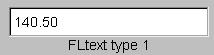
\includegraphics[scale=1]{fltext} 


 FLtext.
 Its value can also be modified by clicking on it and dragging the mouse horizontally. The \emph{istep}
 argument allows the user to arbitrarily set the response on mouse dragging. \subsection*{Examples}


  Here is an example of the fltext opcode. It uses the files \emph{fltext.orc}
 and \emph{fltext.sco}
. 


 \textbf{Example 1. Example of the fltext opcode.}

\begin{lstlisting}
/* fltext.orc */
; A sine with oscillator with fltext box controlled
; frequency either click and drag or double click and
; type to change frequency value
sr = 44100
kr = 441
ksmps = 100
nchnls = 1

FLpanel "Frequency Text Box", 270, 600, 50, 50
    ; Minimum value output by the text box
    imin = 200
    ; Maximum value output by the text box
    imax = 5000
    ; Step size
    istep = 1
    ; Text box graphic type
    itype = 1
    ; Width of the text box in pixels
    iwidth = 70
    ; Height of the text box in pixels
    iheight = 30
    ; Distance of the left edge of the text box 
    ; from the left edge of the panel
    ix = 100
    ; Distance of the top edge of the text box
    ; from the top edge of the panel
    iy = 300

    gkfreq,ihandle FLtext "Enter the frequency", imin, imax, istep, itype, iwidth, iheight, ix, iy
; End of panel contents
FLpanelEnd
; Run the widget thread!
FLrun

instr 1
    iamp = 15000
    ifn = 1
    asig oscili iamp, gkfreq, ifn
    out asig
endin
/* fltext.orc */
        
\end{lstlisting}
\begin{lstlisting}
/* fltext.sco */
; Function table that defines a single cycle
; of a sine wave.
f 1 0 1024 10 1

; Instrument 1 will play a note for 1 hour.
i 1 0 3600
e
/* fltext.sco */
        
\end{lstlisting}
\subsection*{See Also}


 \emph{FLcount}
, \emph{FLjoy}
, \emph{FLkeyb}
, \emph{FLknob}
, \emph{FLroller}
, \emph{FLslider}

\subsection*{Credits}


 Author: Gabriel Maldonado


 New in version 4.22


 Example written by Iain McCurdy, edited by Kevin Conder.
%\hline 


\begin{comment}
\begin{tabular}{lcr}
Previous &Home &Next \\
FLtabsEnd &Up &FLupdate

\end{tabular}


\end{document}
\end{comment}
